\section{Experiments}
\subsection{Datasets}
We also evaluate the performance based on the most typical benchmark on real datasets:
the quantitative structure-activity relationship (QSAR). 
We select Four binary-classification datasets (CPDB, Mutag, AIDS(CAvsCM), CAS) in Table~\ref{tbl:dataset}: 
CPDB and Mutag for mutagenicity tests and AIDS(CAvsCM) for antiviral tests.
All chemical structures are encoded as molecular graphs using RDKit\footnote{\url{http://www.rdkit.org/}}, 
and some structures in the raw data are removed by chemical sanitization\footnote{
Due to this pre-processing, the number of datasets differs from that 
in the simple molecular graphs in the literature, 
where the nodes are labeled by atom type, and the edges are labeled by bond type.}.
We simply apply a node labeling by the RDKit default atom invariants (edges not labeled), i.e., 
atom type, \# of non-H neighbors, \# of Hs, charge, isotope, and inRing properties. 
These default atom invariants use connectivity information similar to that used for the well-known 
ECFP family of fingerprints\cite{Rogers:2010}. See \cite{Kearnes2016} for more elaborate encodings.

\tabcolsep = 6pt
\begin{table}[h]
  \centering
  \caption{Real Dataset summary}
  \label{tbl:dataset}
  	\begin{tabular}{lcccc}
		\thickhline
		Dataset			& CPDB           & Mutag        & AIDS(CAvsCM)     & CAS	\\  \hline
		\# data			& 684            & 188          & 1503             & 4337	\\
		\# ($y=-1,+1$)	& (343, 341)     & (63, 125)    & (1081, 422)      & (1936, 2401)	\\  
		\# nodes		& 25.2           & 26.3         & 59.0             & 30.3	\\  
		\# edges		& 25.6           & 28.1         & 61.6             & 31.3	\\  
		\thickhline
		\end{tabular}
  \leftline{\hspace*{2pt} \# of nodes and edges are average.}
\end{table}

In addition to the real datasets, we also have an artificial datasets.
These artificial datasets are made by randomly sampling 100 graphs from CAS, 
which is one of the real data, and assigning a random label to each graph. 
Artificial1 is assigned as a discrete value labels ($y \in \{-1, +1\}$), 
and Artificial2 is assigned as a real value labels ($y \in [-1, +1]$).
Prepare 100 similar datasets for each.
These summary is shown in Table~\ref{tbl:artificial}.
These are used to more generally evaluate each search policy, 
taking into account the settings and properties of various problems.


\tabcolsep = 20pt
\begin{table}[h]
  \centering
  \caption{Artificial Dataset summary}
  \label{tbl:artificial}
  	\begin{tabular}{lcc}
		\thickhline
		Dataset			& Artificial1           & Artificial2        \\  \hline
		\# data			& 100            		& 100          \\
		\# dataset		& 100     	 			& 100    	\\  
		$y$				& $\{-1, +1\}$     	 	& $[-1, +1]$    	\\  
		sampled from			& CAS     	 			& CAS    	\\  
		\thickhline
		\end{tabular}
\end{table}

\subsection{Comparison of Respective Search Efficiency}
First, a feature search is performed once for each artificial dataset without any budget constraint, 
thereby comparing the respective search efficiencies.
Exploration strength parameter of MCTS is set with three type of values (0.1, 1, 10).
Figure~\ref{fig:bestsearch}, \ref{fig:update} are the average results for all 100 datasets, 
which show the number of nodes searched until finding the best subgraph pattern 
and how the provisional solution is updated in each search.
Figure~\ref{fig:bestsearch} shows that MCTS find the best subgraph with the minimum number of searches, 
and the best-first search continues at that point.
In addition, it was found that each search was not significantly affected by the type of graph label, 
and the smaller the value of the MCTS parameter, the better the result.

In Figure~\ref{fig:update}, both of the proposed methods 
can find a good solution faster than the existing depth-first search.
Also the solution is rapidly improved and converged at an early step, 
there is a sufficient expectation for an approximate search under fixed budget constraint.

\begin{figure}[htbp]
 \begin{minipage}{0.5\hsize}
  \begin{center}
   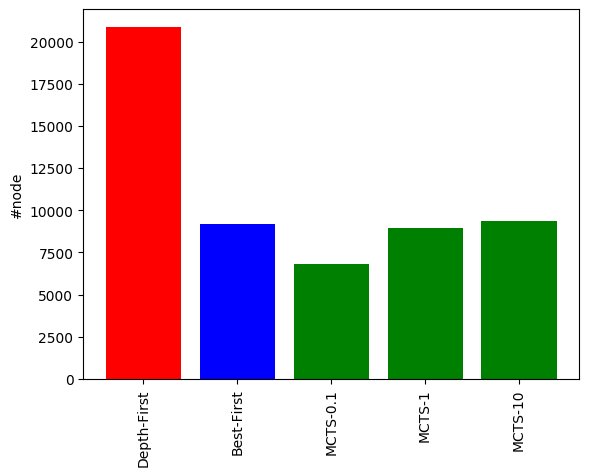
\includegraphics[width=63mm]{img/cas/artificial/1/node.png}
  \end{center}
  \subcaption{Artificial1 ($y \in \{-1, +1\}$)}
 \end{minipage}
 \begin{minipage}{0.5\hsize}
  \begin{center}
   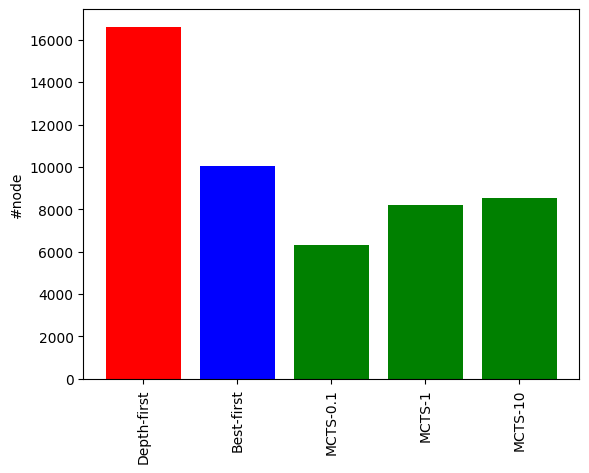
\includegraphics[width=63mm]{img/cas/artificial/2/node.png}
  \end{center}
  \subcaption{Artificial2 ($y \in [-1, +1]$)}
 \end{minipage}
 \caption{Cost comparison until finding the best solution.}
  \label{fig:bestsearch}
\end{figure}

\begin{figure}[htbp]
 \begin{minipage}{0.5\hsize}
  \begin{center}
   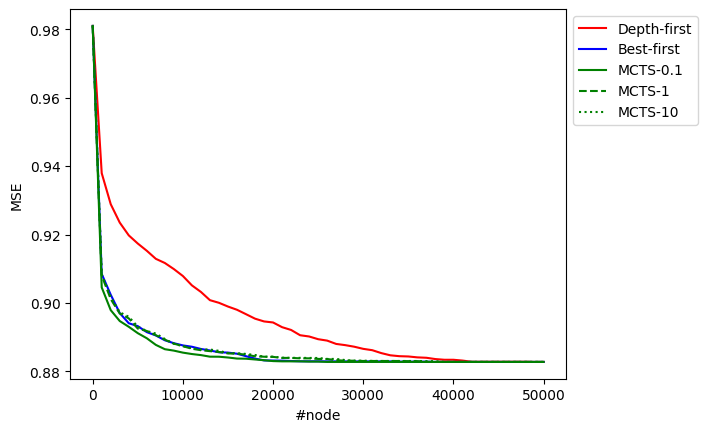
\includegraphics[width=65mm]{img/cas/artificial/1/node_chart.png}
  \end{center}
  \subcaption{Artificial1 ($y \in \{-1, +1\}$)}
 \end{minipage}
 \begin{minipage}{0.5\hsize}
  \begin{center}
   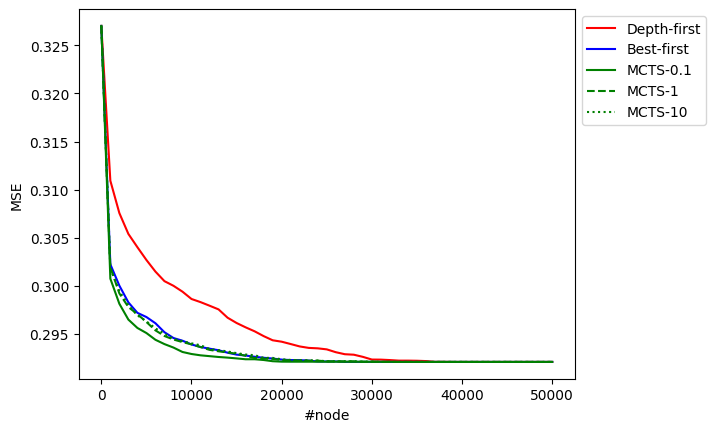
\includegraphics[width=65mm]{img/cas/artificial/2/node_chart.png}
  \end{center}
  \subcaption{Artificial2 ($y \in [-1, +1]$)}
 \end{minipage}
 \caption{Comparison of update of provisional solution.}
  \label{fig:update}
\end{figure}

\subsection{Gradient Tree Boosting with Approximate Search for QSAR}
\label{sec:qsar}
Now that the search efficiency of the proposed method has been confirmed, 
in this part, we construct gradient tree boosting (GTB) \cite{Shirakawa:2018} model for QSAR datasets 
using iterative approximate search of the discriminating subgraphs under fixed budget constraint.
GTB parameters are fixed at the following values,
max subgraph size is 10, the number of trees is 100, depth of each trees is 1 and shrinkage is 1.
The budget constraint on the search is set to 
CPDB=(1000, 2000, 3000, 4000, 5000), Mutag=(200, 400, 600, 800, 1000), 
AIDS(CAvsCM)=(1000, 2000, 3000, 4000, 5000) and CAS=(5000, 10000, 15000, 20000, 25000), 
according to the scale of the dataset, 
and the search is terminated when the number of search nodes exceeds the budget.
The results in Figures~\ref{fig:trainloss} \ref{fig:acc_node} and \ref{fig:acc_time} 
were measured by 10-fold cross validation, 
and Figure~\ref{fig:frequency_time} was measured using all CAS data.

Figure~\ref{fig:trainloss} shows the change in training loss 
of the final ensemble model to the search budget constraint.
Comparing the learning of the model with the same number of searches, 
it can be seen that the model using MCTS performed the best.
For the MCTS exploration strength parameter, 
the same performance is shown, despite the fact that the difference is up to 100 times, 
indicating that the search is robust to this parameter.
The result of the accuracy, is shown in Figure~\ref{fig:acc_node}, 
is similar to the result of the training loss, 
and the accuracy of the model using the MCTS is the highest. 
On the other hand, the approximation search based on the existing depth-first policy 
resulted in poor model accuracy.

Then, we consider the execution time.
Figure~\ref{fig:acc_time} indicates that 
the best-first search requires the longest execution time. 
On the other hand, the execution time of the depth-first search 
is very fast for the same number of searches.
In order to verify this difference in execution time, 
consider the properties of the subgraphs searched by each method.
Figure~\ref{fig:frequency_time} shows the average frequency of the subgraphs searched 
by each method and the execution time.
From Figure~\ref{fig:frequency_time} (a), it can be seen that the subgraphs searched by best-first policy 
have an average frequency 30 times higher than depth-first and 4 times higher than MCTS.
Looking at the lower bound (\ref{eq:bound_R}) in the previous section \ref{sec:previous}, 
the graph with the higher frequency has a larger maximum value of $k$, 
and the lower bound is likely to be larger 
because the movement pattern of many sets can be considered.
In addition, the depth-first policy likely to search for many large subgraphs, 
but the frequency of those is generally low.
Since the calculation of the lower bound requires a linear cost for the frequency, 
there is a large difference in the execution time like Figure~\ref{fig:frequency_time} (b).
The hatched portion of Figure~\ref{fig:frequency_time} (b) indicates the computational cost 
other than the lower bound, and the other portion indicates the computational cost of the bound.
Even if the execution time differs for such a reason, 
the MCTS model showed the best performance 
when the accuracy of the model was evaluated at the same execution time.

\begin{figure}[htbp]
 \begin{minipage}{0.5\hsize}
  \begin{center}
   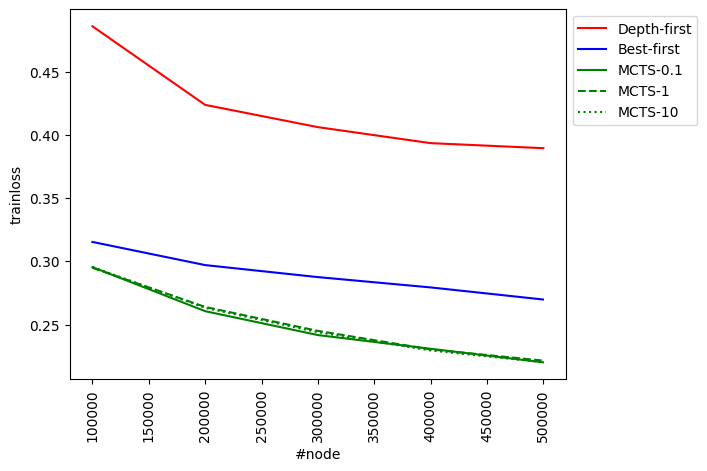
\includegraphics[width=65mm]{img/cpdb/grid/trainloss_node.png}
  \end{center}
  \subcaption{CPDB}
 \end{minipage}
 \begin{minipage}{0.5\hsize}
  \begin{center}
   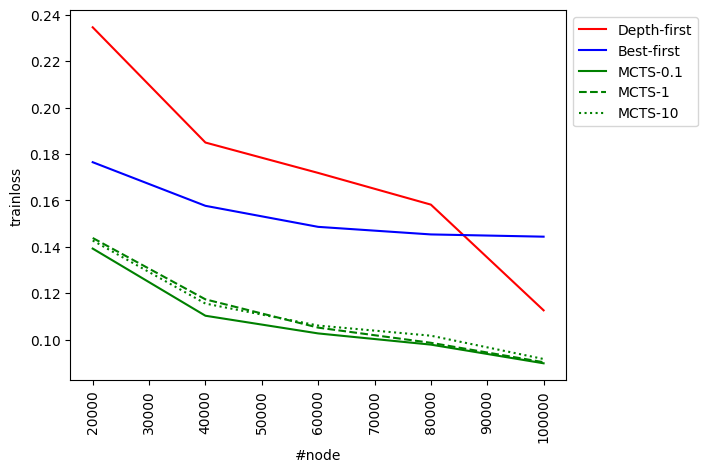
\includegraphics[width=65mm]{img/mutag/grid/trainloss_node.png}
  \end{center}
  \subcaption{Mutag}
 \end{minipage}\\
 \begin{minipage}{0.5\hsize}
  \begin{center}
   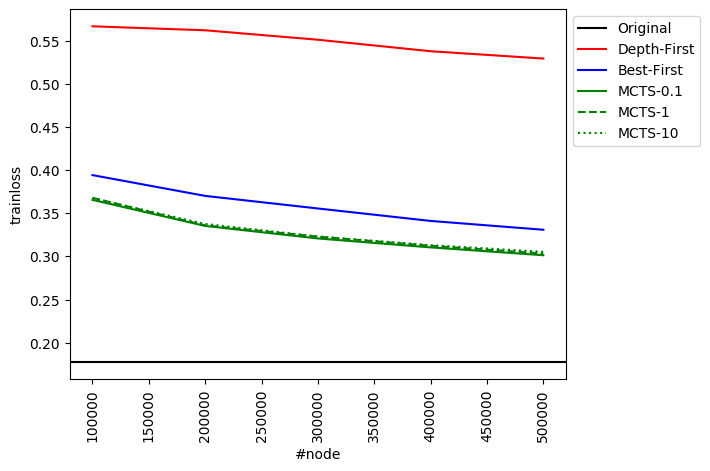
\includegraphics[width=65mm]{img/aids/grid/trainloss_node.png}
  \end{center}
  \subcaption{AIDS}
 \end{minipage}
 \begin{minipage}{0.5\hsize}
  \begin{center}
   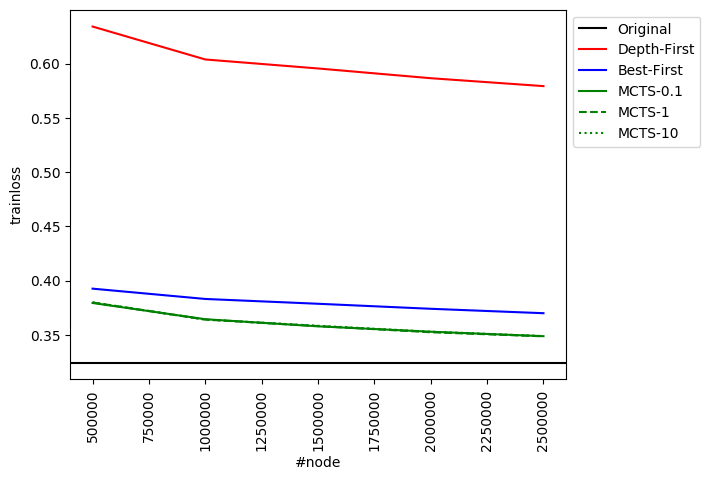
\includegraphics[width=65mm]{img/cas/grid/trainloss_node.png}
  \end{center}
  \subcaption{CAS}
 \end{minipage}
 \caption{Training loss to the number of search nodes for QSAR.}
  \label{fig:trainloss}
\end{figure}

\begin{figure}[htbp]
 \begin{minipage}{0.5\hsize}
  \begin{center}
   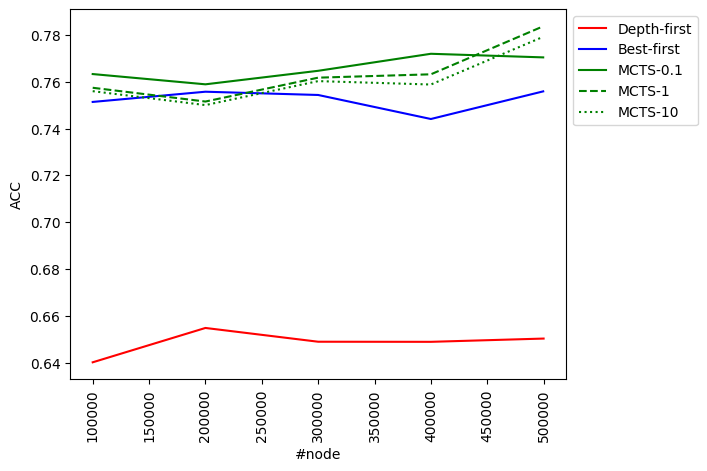
\includegraphics[width=65mm]{img/cpdb/grid/acc_node.png}
  \end{center}
  \subcaption{CPDB}
 \end{minipage}
 \begin{minipage}{0.5\hsize}
  \begin{center}
   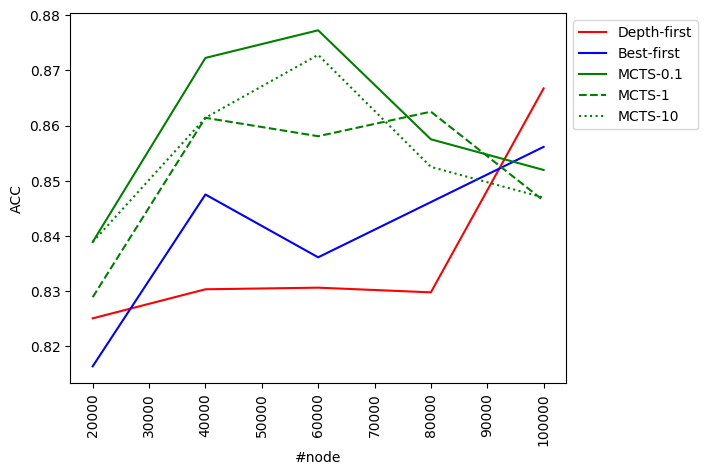
\includegraphics[width=65mm]{img/mutag/grid/acc_node.png}
  \end{center}
  \subcaption{Mutag}
 \end{minipage}\\
 \begin{minipage}{0.5\hsize}
  \begin{center}
   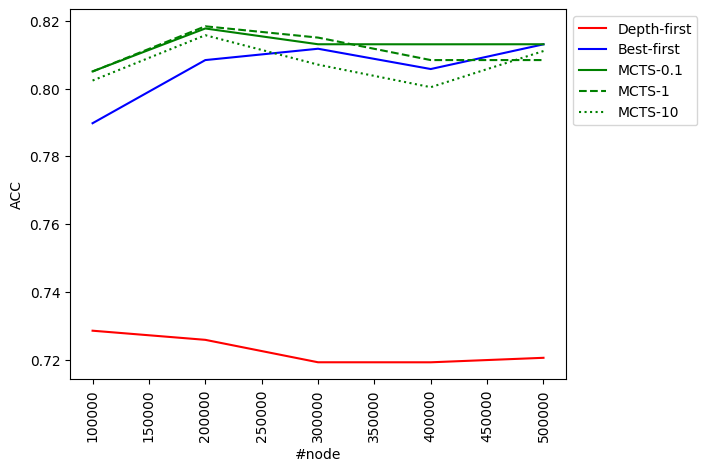
\includegraphics[width=65mm]{img/aids/grid/acc_node.png}
  \end{center}
  \subcaption{AIDS}
 \end{minipage}
 \begin{minipage}{0.5\hsize}
  \begin{center}
   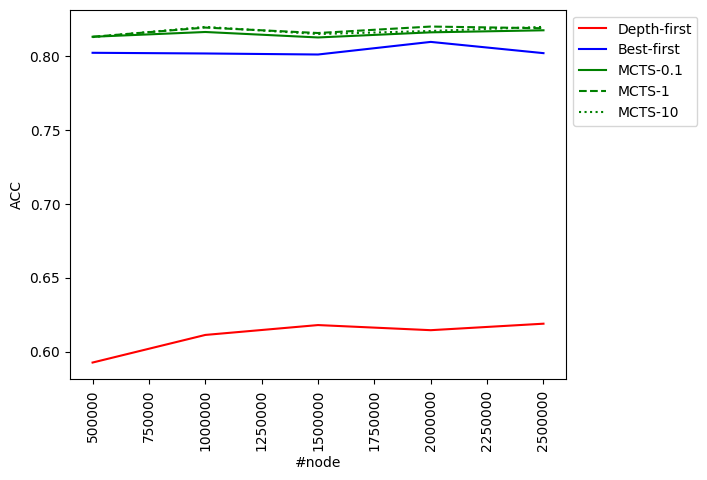
\includegraphics[width=65mm]{img/cas/grid/acc_node.png}
  \end{center}
  \subcaption{CAS}
 \end{minipage}
 \caption{Test accuracy to the number of search nodes for QSAR.}
  \label{fig:acc_node}
\end{figure}

\begin{figure}[htbp]
 \begin{minipage}{0.5\hsize}
  \begin{center}
   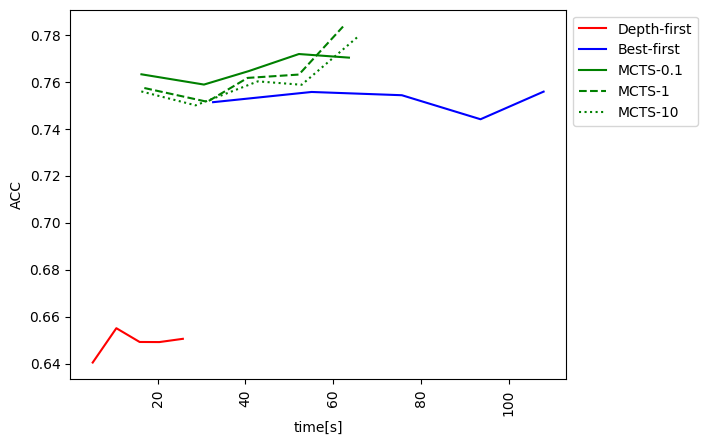
\includegraphics[width=65mm]{img/cpdb/grid/acc_time.png}
  \end{center}
  \subcaption{CPDB}
 \end{minipage}
 \begin{minipage}{0.5\hsize}
  \begin{center}
   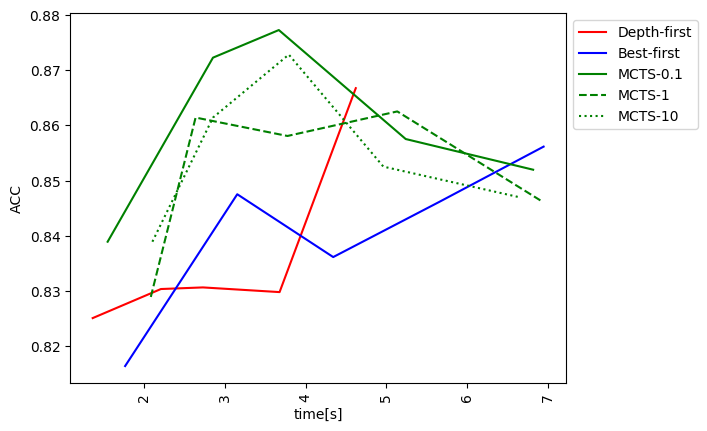
\includegraphics[width=65mm]{img/mutag/grid/acc_time.png}
  \end{center}
  \subcaption{Mutag}
 \end{minipage}\\
 \begin{minipage}{0.5\hsize}
  \begin{center}
   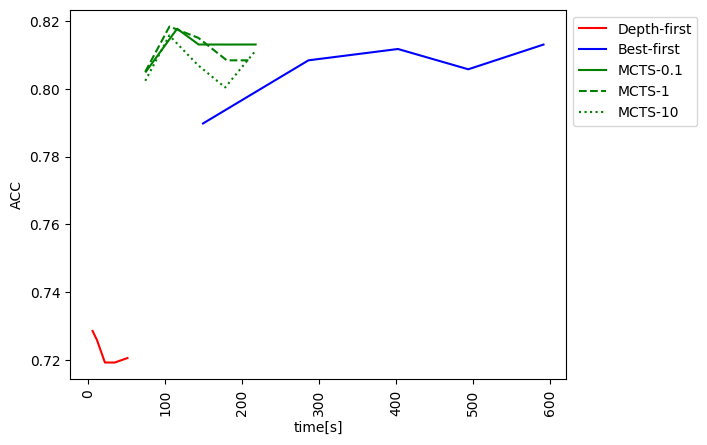
\includegraphics[width=65mm]{img/aids/grid/acc_time.png}
  \end{center}
  \subcaption{AIDS}
 \end{minipage}
 \begin{minipage}{0.5\hsize}
  \begin{center}
   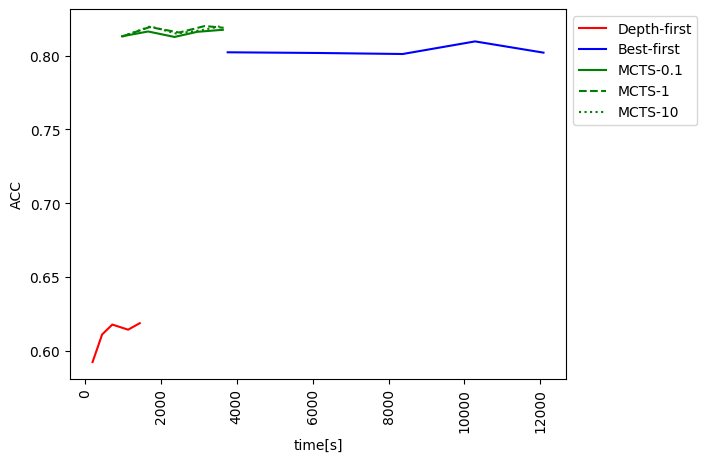
\includegraphics[width=65mm]{img/cas/grid/acc_time.png}
  \end{center}
  \subcaption{CAS}
 \end{minipage}
 \caption{Test accuracy to execution time for QSAR.}
  \label{fig:acc_time}
\end{figure}

\begin{figure}[htbp]
 \begin{minipage}{0.5\hsize}
  \begin{center}
   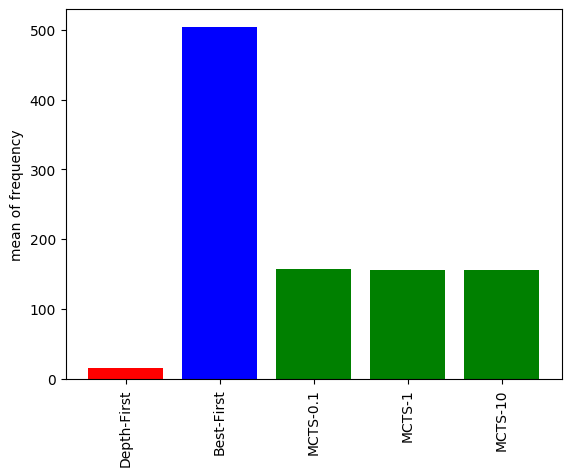
\includegraphics[width=65mm]{img/frequency.png}
  \subcaption{Average frequency of searched subgraphs.}
  \end{center}
  \label{fig:frequency}
 \end{minipage}
 \begin{minipage}{0.5\hsize}
  \begin{center}
   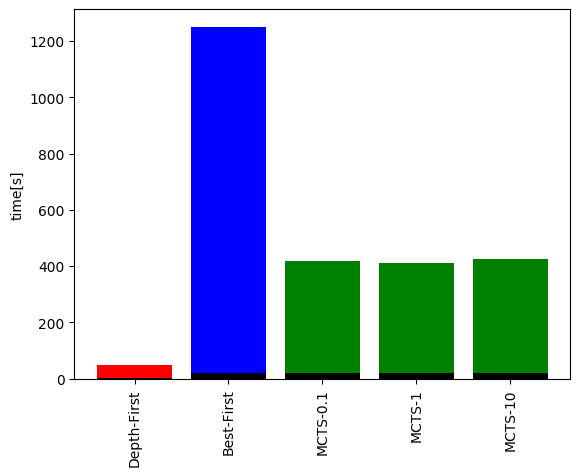
\includegraphics[width=65mm]{img/time.png}
  \subcaption{Execution time of each search.\\ }
  \end{center}
  \label{fig:time}
 \end{minipage}
 \caption{Relationship between execution time and frequency of searched subgraphs for CAS.}
  \label{fig:frequency_time}
\end{figure}

\subsection{Approximate Search vs. Exact Search for Learning}
So far, we have considered the efficiency of each approximate search.
Then, we compare the approximate search with the exact search.
Since approximate search based on MCTS policy performed the best 
compared with other approximate search methods, 
this section compares GTB+MCTS with the existing method \cite{Shirakawa:2018}, GTB+exact Depth-first
The same parameters of GTB and budget constraint are used as for \ref{sec:qsar}
and compared using the test accuracy of 10-fold cross-validation for QSAR datasets.
The results are shown in Table~\ref{tbl:acc} 
and the best MCTS parameters used in the results are shown in Table~\ref{tbl:bestParam}.
Table~\ref{tbl:acc} shows that, the accuracy of GTB+MCTS was $0.4\%~2.7\%$ higher than 
the accuracy of GTB+exact Depth-first.
In addition, the number of search nodes and execution time were reduced from about $1/10$ to $1/200$.
Why did the accuracy of learning improve despite under budget constrain?
Figure~\ref{fig:feature_rate} shows the answer.
This figure indicates the percentage of subgraph size used for learning,
and it can be seen that model based on the exact Depth-first is learned with almost large features.
In particular, 40\% or more of the maximum size feature is used.
This is apparently over-fitting and led to a decrease in accuracy.
On the other hand, model based on MCTS (approximate search) is built with a good balance of features.
The latter is considered to be a better model in terms of generalization performance.

\tabcolsep = 10pt
\begin{table*}[t]
  \centering
  \caption{exact Depth-first vs. MCTS (approximate search).}
  \label{tbl:acc}
  \scalebox{0.90}{
  	 \begin{tabular}{lccc}
  	   \thickhline
  	   Dataset		& ~								& \# Search nodes					& ~			\\
  	   ~   			& GTB+exact Depth-first			& GTB+MCTS       			& Ratio \\ \hline
  	   CPDB 		& $7.2 \times 10^6$				& $5.0 \times 10^5$ 				&  $0.070$  \\
  	   Mutag 		& $3.8 \times 10^5$				& $6.0 \times 10^4$ 				&  $0.015$  \\
  	   AIDS(CAvsCM)	& $7.9 \times 10^7$				& $2.0 \times 10^5$ 				&  $0.003$  \\
  	   CAS	 		& $6.9 \times 10^7$				& $2.0 \times 10^6$ 				&  $0.029$  \\
  	   \thickhline
  	  		 		& ~								& Execution time [s]				& ~			\\
  	   ~   			& GTB+exact Depth-first			& GTB+MCTS       			& Ratio \\ \hline
  	   CPDB 		& $8.2 \times 10^2$				& $6.2 \times 10$	 				&  $0.076$  \\
  	   Mutag 		& $2.3 \times 10^2$				& $3.7$				 				&  $0.016$  \\
  	   AIDS(CAvsCM)	& $2.5 \times 10^4$				& $1.1 \times 10^2$ 				&  $0.004$  \\
  	   CAS	 		& $8.0 \times 10^4$				& $1.7 \times 10^3$ 				&  $0.040$  \\
  	   \thickhline
  	   				& ~								& Accuracy [\%]						& ~			\\
  	   ~   			& GTB+exact Depth-first			& GTB+MCTS       			& Difference \\ \hline
  	   CPDB 		& $77.78$						& $78.35$			 				&  $+0.57$  \\
  	   Mutag 		& $85.03$						& $87.73$			 				&  $+2.70$  \\
  	   AIDS(CAvsCM)	& $81.37$						& $81.84$ 							&  $+0.47$  \\
  	   CAS	 		& $80.82$						& $81.99$		 					&  $+1.17$  \\
  	   \thickhline
  	 \end{tabular}
  }
\end{table*}

\tabcolsep = 14pt
\begin{table*}[t]
  \centering
  \caption{Best budget constraint and exploration strength parameter.}
  \label{tbl:bestParam}
  	\scalebox{0.90}{
  	\begin{tabular}{lcccc}
  	  \thickhline
  	  ~                    	& CPDB     	& Mutag 	& AID(CAvsCM) 	& CAS  		\\  \hline
  	  budget constraint    	& $5000$ 	& $600$ 	& $2000$  		& $20000$		\\  
  	  exploration strength  & $1$ 		& $0.1$		& $1$ 	 		& $1$			\\ 
  	  \thickhline
  	\end{tabular}
  }
\end{table*}

\begin{figure}[htbp]
  \begin{center}
   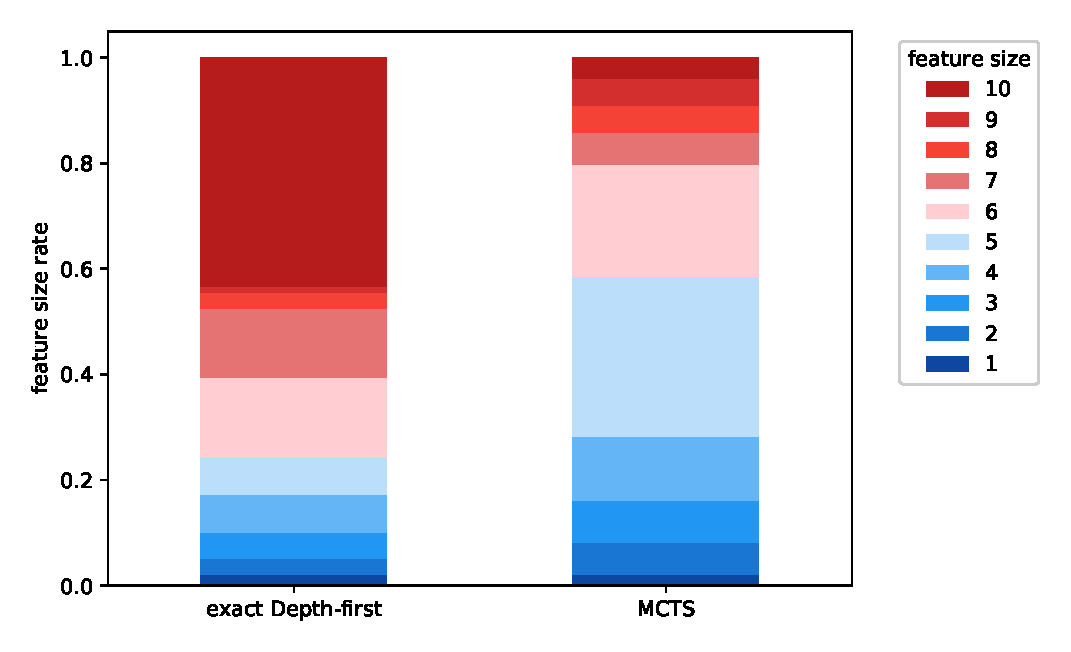
\includegraphics[width=95mm]{img/feature_rate.eps}
  \end{center}
 \caption{The size ratio of the features used for learning the MCTS (approximate search) and the exact Depth-first search.}
  \label{fig:feature_rate}
\end{figure}

